
\section{Introduction}

\subsection{Crane presentation and control goals}

\begin{frame}{The crane System}
\framesubtitle{Real Crane}
\begin{figure}
    \centering
    \rotatebox{270}{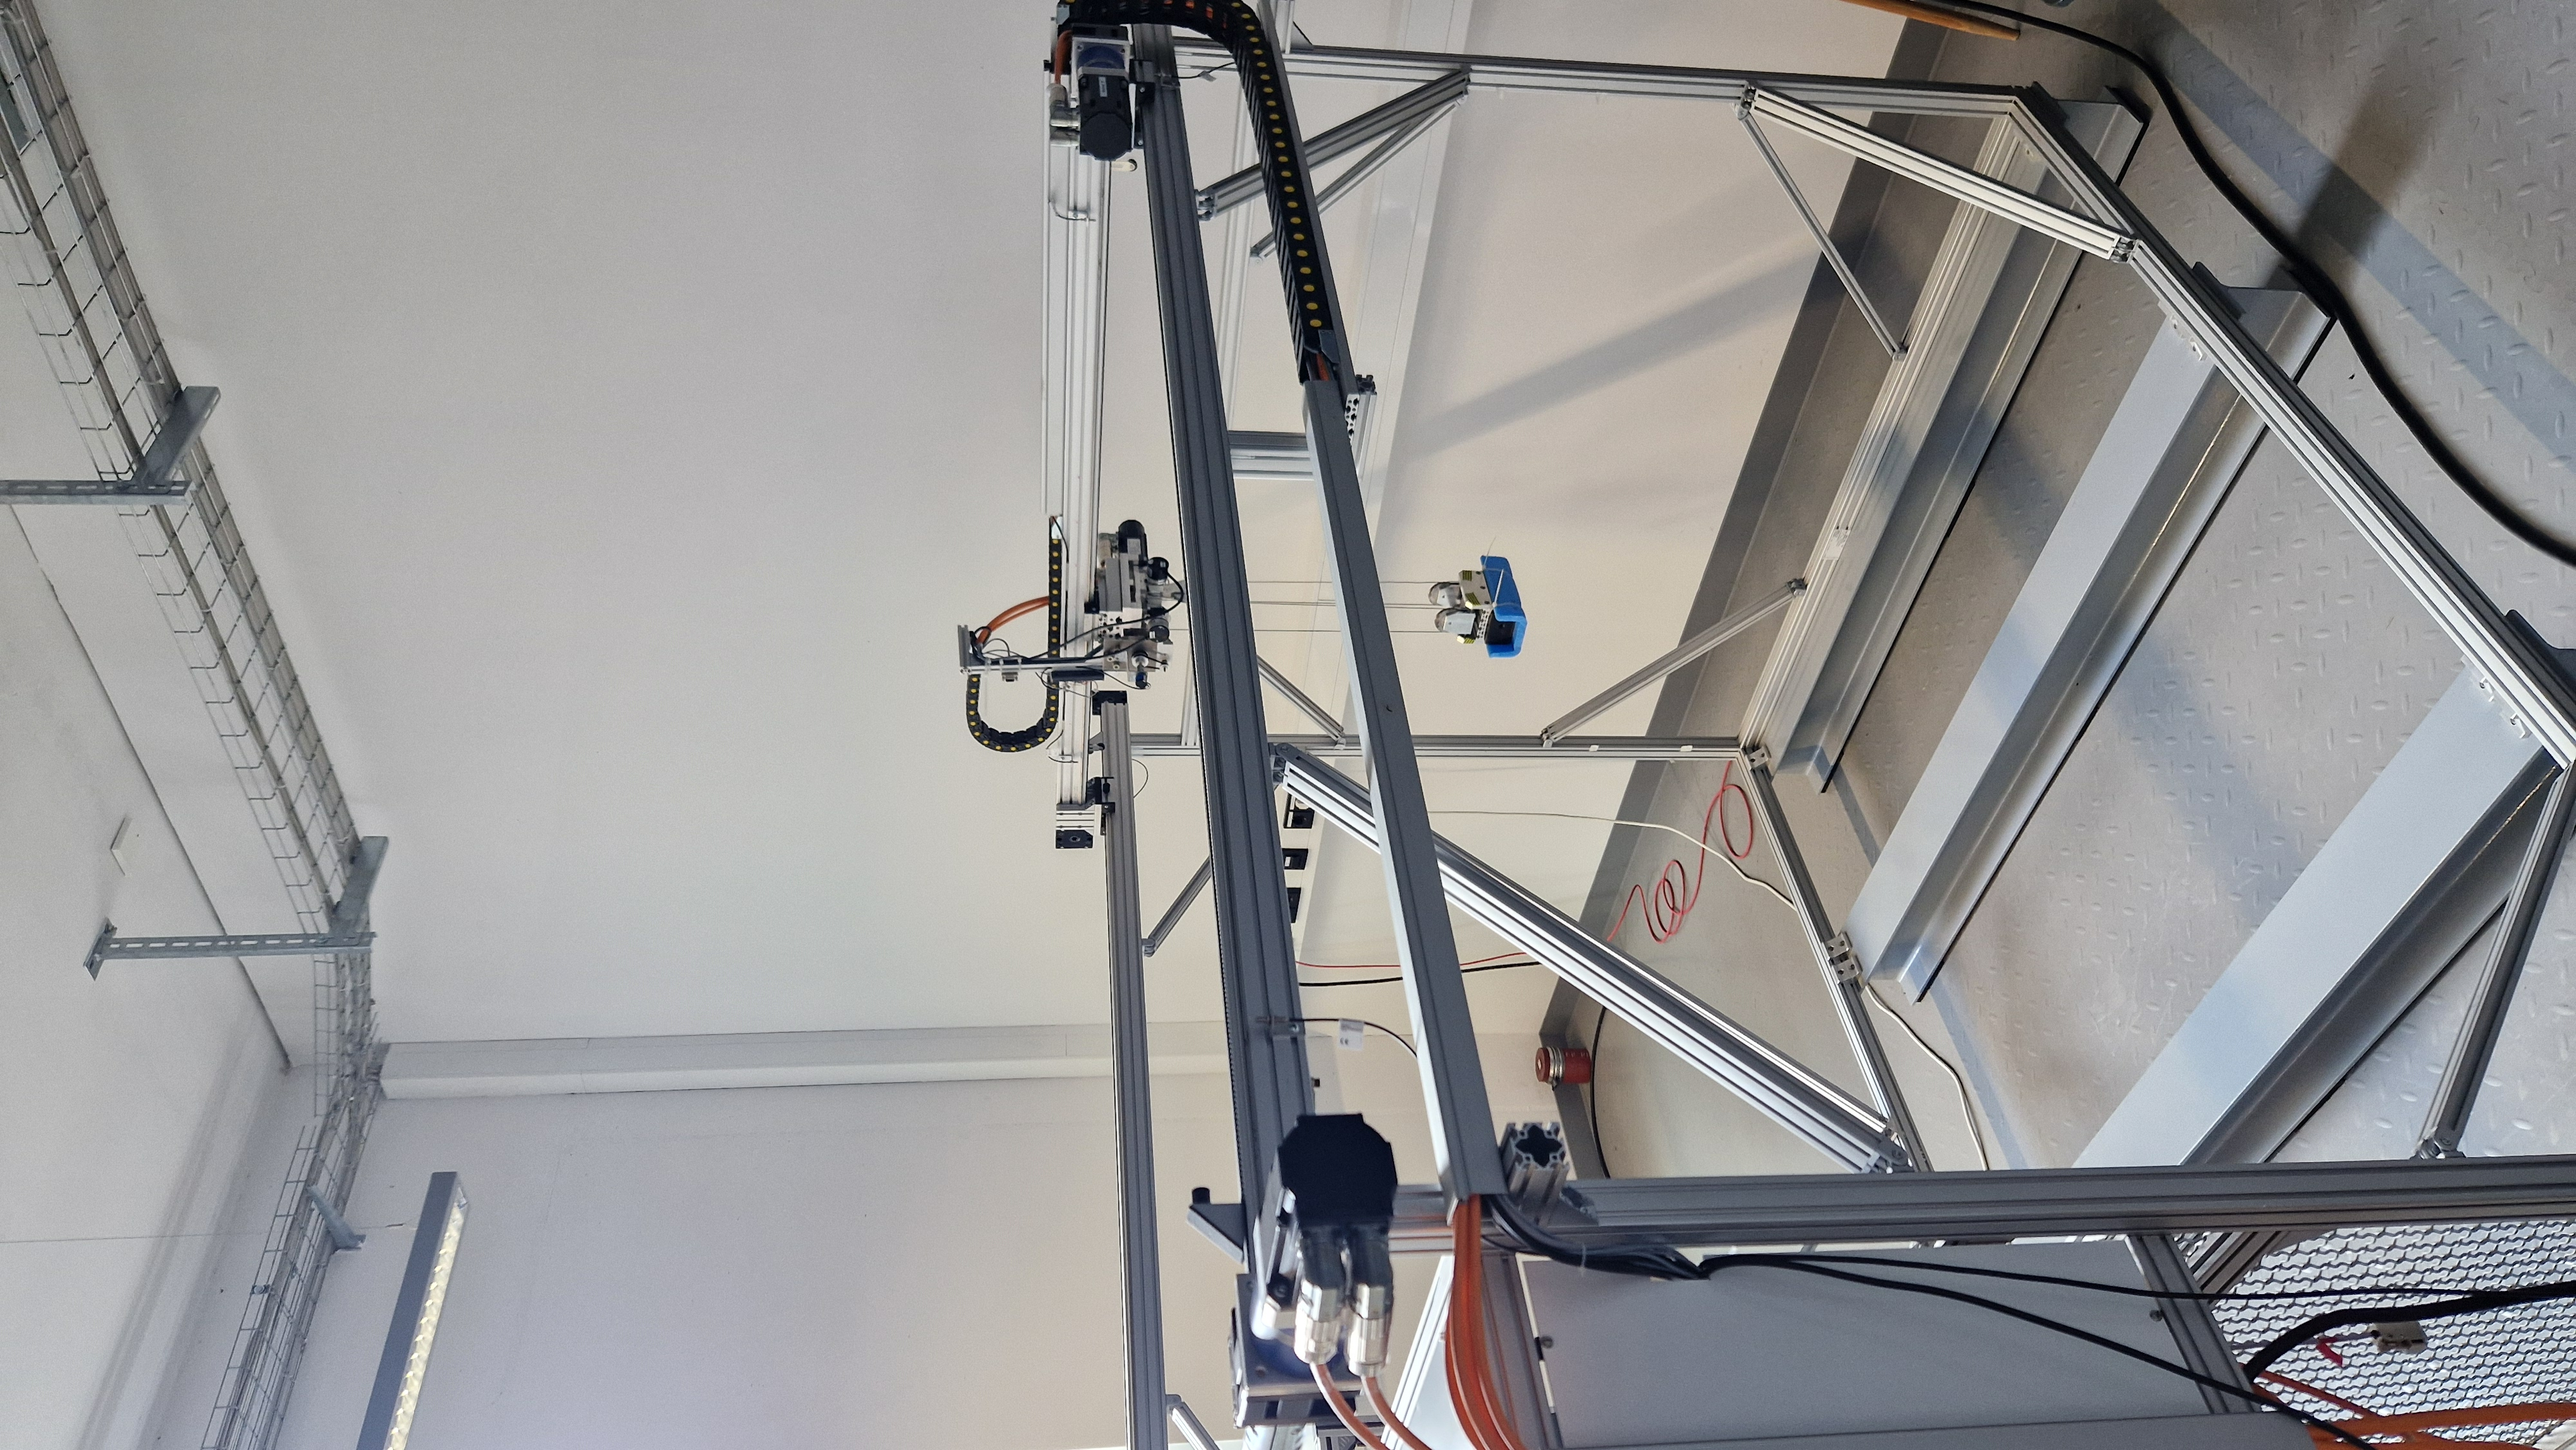
\includegraphics[width=0.5\linewidth]{imgs/Simulation/General.jpg}}
    \caption{Real 3-dim overhead Crane}
\end{figure}
\end{frame}



\begin{frame}{The crane System}
\framesubtitle{Scheme}
    \begin{figure}
        \centering
        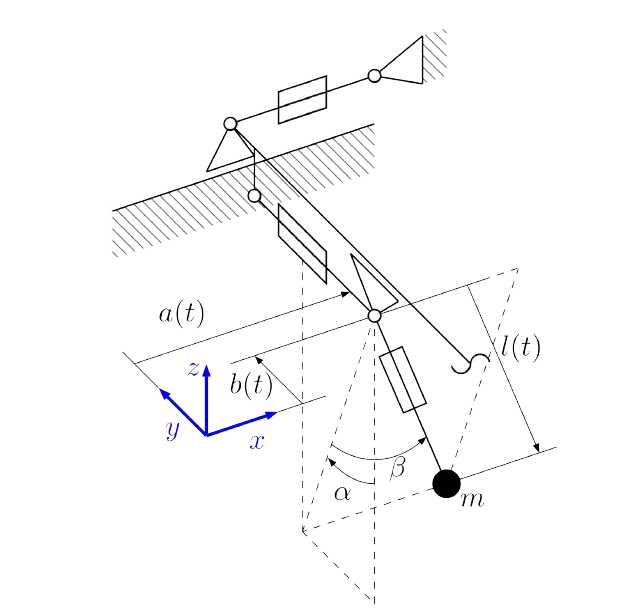
\includegraphics[width=0.5\linewidth]{imgs/Crane/3DimCranSchem.PNG}
        \caption{Schematics of three dimensional overhead crane \cite{Knierim2010Crane}}
        \label{fig:Schematics of three dimensional overhead crane}
    \end{figure}
\end{frame}

\begin{frame}{Control Goals}
     The goals of this work are : 
    \begin{itemize}
        \item Implement a Model Following Control (MFC) to make the crane's load track set points and trajectories 
        \item Highlight the attenuation of the peaking phenomenon by the MFC
    \end{itemize}

\end{frame}


%______________________________________________________________________________%
\section{Crane Overview}
\subsection{Crane Model}
\begin{frame}{The Trolley}
\begin{columns}[T]
    \begin{column}{0.5\textwidth}
        \centering
        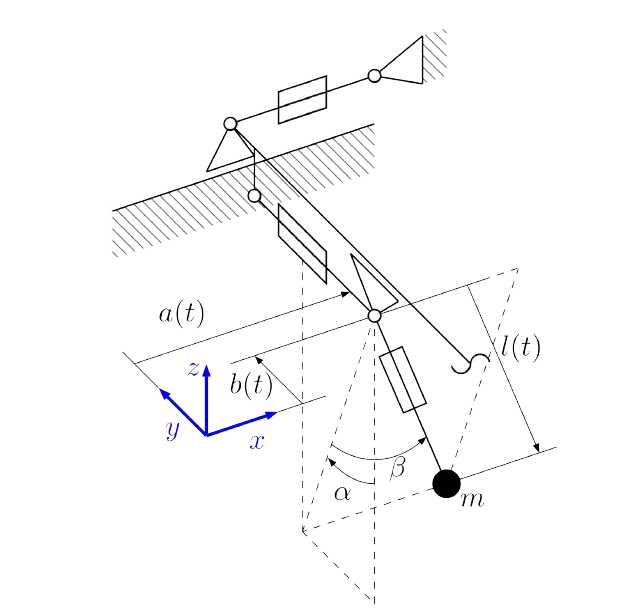
\includegraphics[width=\linewidth]{imgs/Crane/3DimCranSchem.PNG}
        \captionof{figure}{Schematics of three dimensional overhead crane \cite{Knierim2010Crane}}
        \label{fig:Schematics of three dimensional overhead crane}
    \end{column}
    \begin{column}{0.5\textwidth}
        First, the crane dynamic equations are computed as in \cite{Knierim2010Crane}. The trolley position \(\boldsymbol{r}_{t}(t)\) is considered as a time-dependent function given by:

         \vspace{1em} % Add vertical space
         
        \begin{equation}
            \textbf{r}_t(t) = \begin{bmatrix}
                a(t) & b(t) & 0
            \end{bmatrix}^T
        \end{equation}

         \vspace{1em} % Add vertical space
         
        where \(a(t)\) and \(b(t)\) are the positions of the trolley in the \(x\) and \(y\) directions.
    \end{column}
\end{columns}
\end{frame}


\begin{frame}{System output}
\begin{columns}[T]
\begin{column}{0.5\textwidth}
        \centering
        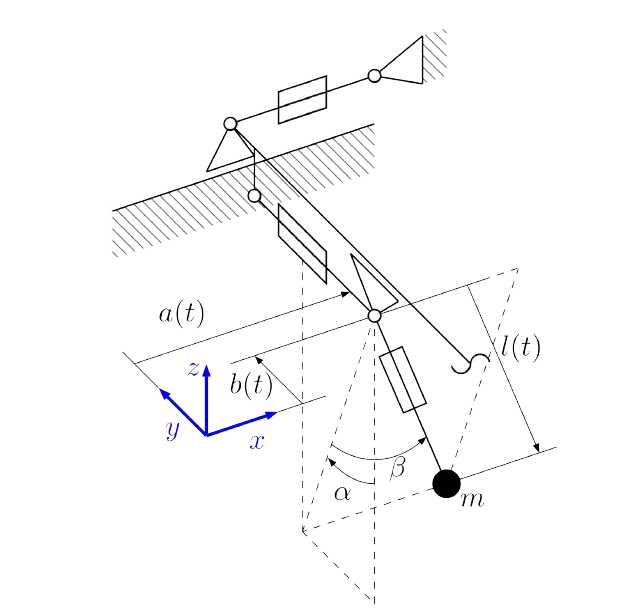
\includegraphics[width=\linewidth]{imgs/Crane/3DimCranSchem.PNG}
        \captionof{figure}{Schematics of three dimensional overhead crane \cite{Knierim2010Crane}}
        \label{fig:Schematics of three dimensional overhead crane}
\end{column}
    
\begin{column}{0.5\textwidth}
    The position of the load, which will be the output of the system as \(\textbf{y}(t)\) given by :

 \vspace{1em} % Add vertical space
 
\begin{equation}
    \textbf{y}(t) = \begin{bmatrix}
        a(t) + l(t)S_\beta \\
    b(t) + l(t)C_\beta S_\alpha \\
    -l(t)C_\beta C_\alpha
    \end{bmatrix}
\end{equation}

 \vspace{1em} % Add vertical space
 

With the notations \(S_\gamma = sin(\gamma)\) and \(C_\gamma = cos(\gamma)\).
\end{column}

\end{columns}

\end{frame}

\begin{frame}{Dynamic Equation}
 We define the generalized coordinates vector \(\boldsymbol{\theta} = \left[ \alpha \; \beta \right]^T\) to get the Newton-Euler equation of the load system. 

 First let's note  \( \boldsymbol{J}_{l}(t)\), the jacobian of the crane over the generalized coordinates : 

\begin{equation}
     \boldsymbol{J}_{l}(t) = \frac{\partial \boldsymbol{y}(t)}{\partial \boldsymbol{\theta}} = \begin{bmatrix}
         0                       & l(t)C_\beta \\
         l(t)C_\beta C_\alpha    & -l(t)S_\beta S_\alpha \\
         l(t)C_\beta S_\alpha    & l(t)S_\beta C_\alpha
     \end{bmatrix}
\end{equation}
\end{frame}

\begin{frame}{Dynamic Equation}
The velocity and acceleration of the load are given by : 
\begin{align}
    \dot{\boldsymbol{y}} &= \boldsymbol{J}_{l}(t) \dot{\theta} + \underbrace{ \left. \frac{\partial \boldsymbol{y}}{\partial t} \right\|_{\theta=cst}}_{\bar{\dot{\boldsymbol{y}}}(t)} \\
    \ddot{\boldsymbol{y}} &= \boldsymbol{J}_{l}(t) \ddot{\theta} + \underbrace{\frac{d\boldsymbol{J}_{l}(t)}{dt} \cdot \dot{\boldsymbol{\theta}} + \frac{d\bar{\dot{\boldsymbol{y}}}(t)}{dt}}_{\bar{\ddot{\boldsymbol{y}}}(t)}
\end{align}
\end{frame}

\begin{frame}{Crane Model Overview}
    After some steps and by applying the Newton-Euler equation, the system reads :
    \begin{equation}
\label{eq:equation_of_motion_generalized_coordinates}
    \boldsymbol{J}_{l}(t)^T\boldsymbol{J}_{l}(t)\cdot \ddot{\boldsymbol{\theta}} = -\boldsymbol{J}_{l}(t)^T \: \bar{\ddot{\boldsymbol{y}}}(t) \; + \; \boldsymbol{J}_{l}(t)^T\boldsymbol{g}
\end{equation}

Where \(\boldsymbol{g} = \begin{bmatrix} 0 & 0 & -g\end{bmatrix}^T\) denotes the gravity vector.
\end{frame}

\begin{frame}{Dynamic Equation}
 The input is be the same as in the simulation and the real crane experimentation, they will directly drive the \(\begin{bmatrix}\ddot{a}(t) & \ddot{b}(t) & \ddot{l}(t)\end{bmatrix}\) coordinates. Which gives us the complete dynamics of the crane plant system in the form of a non-linear vectorial second order differential equation \cite{Knierim2010Crane} : 


\begin{align}
\left\{ \begin{array}{ll}
\ddot{a}(t) &= u_1\\ 
\ddot{b}(t) &= u_2\\ 
\ddot{l}(t) &= u_3\\
\ddot{\alpha}(t) &= \frac{1}{l(t) C_{\beta}} \left(2 \dot{\alpha} \dot{\beta} S_{\beta} l(t) - 2 \dot{l}(t) \dot{\alpha} C_{\beta} - S_{\alpha} g - C_{\alpha} u_2\right) \\
\ddot{\beta}(t) &= \frac{1}{l(t)} \left(-C_{\alpha} S_{\beta} g - S_{\beta} C_{\beta} \dot{\alpha}^2 l(t) - 2 \dot{l}(t) \dot{\beta} + S_{\beta} S_{\alpha} u_2 - C_{\beta} u_1\right) \\
\end{array}
\right.
\end{align}

and the output :  \(\textbf{y}(t) \)

\end{frame}

\begin{frame}{Dynamic Equation}
 We can now write this system into the normal form : 

\begin{align*}
    \dot{\boldsymbol{x}} &= \boldsymbol{f}(\boldsymbol{x}) + \boldsymbol{g}(\boldsymbol{x})\boldsymbol{u} \\
     \boldsymbol{y}  &= \boldsymbol{h}(\boldsymbol{x})
\end{align*}

where : 
\begin{align*}
    \boldsymbol{x}(t) &= (x_i(t))_{1\le i\le 10} \\ &= \begin{pmatrix} a(t) & \dot{a}(t) & b(t) & \dot{b}(t) & l(t) & \dot{l}(t) & \alpha(t) & \dot{\alpha}(t) & \beta(t) & \dot{\beta}(t)\end{pmatrix}^T
\end{align*}
Denotes the state vector

It is required for a system to be in Byrnes-Isidori to apply MFC. Exact feedback linearization is used in this MIMO system.
\end{frame}
%_______________________________________________________________________%

\subsection{Feedback linearization and dynamic extension}

\begin{frame}{Dynamic Extension}

The Feedback linearization applied directly to the crane equation has internal dynamics. One solution is to artificially increase the relative degree of \(y_3\) by implementing a dynamic extension as in \cite{Noack2020} by introducing a virtual control input that reads : 
\begin{align}
    \ddot{\nu} &= w_3 \\
    u_3 &= \psi(\boldsymbol{x}, \nu)
\end{align}

\(u_3\) is computed so that \(
    \forall t \ge 0 \; , \quad \ddot{y}_3(t) - \nu(t) = 0\) 
\end{frame}



\begin{frame}{Feedback Linearization}
   \begin{itemize}
       \item  With our crane system, the relative degrees of our outputs \([y_1, y_2, y_3]^T\) are respectively \([2, 2, 2]^T\), which leads to internal dynamics. 

       \item One way to address this issue is to artificially increase the relative degree of \(y_3\) by applying the previous dynamical extension that has in our case the propriety ti increase the relative degrees to  \([4, 4, 4]^T\).
   \end{itemize}
\end{frame}


\begin{frame}{Feedback Linearization}
    Now it can be shown that by applying the following transformation to each output \(y_i\) for \(i \in \{1, 2, 3\}\) of the system,

\begin{equation}
\boldsymbol{\xi}_i
=
\boldsymbol{T}_i(\boldsymbol{x})
=
\begin{bmatrix}
    y_i \\
    \dot{y}_i \\
    \ddot{y}_i \\
    y^{(3)}_i
\end{bmatrix}
\end{equation}

The system is divided into 3 decoupled subsystems in Byrnes-Isidori form that read : 

\begin{equation}
\label{eq:flat_sys_reduced}
\forall i \in \{1, 2, 3\} : 
\left\{
\begin{aligned}
  \dot{\boldsymbol{\xi}_i} &= \boldsymbol{A} \boldsymbol{\xi}_i + \boldsymbol{B} \big(a_i(\boldsymbol{\xi}) + b_i(\boldsymbol{\xi})u)\\
  \boldsymbol{y}_i &= \boldsymbol{C} \boldsymbol{\xi}_i 
\end{aligned}
\right.
\end{equation}
\end{frame}



